\section{Deploying on Volc\'{a}n Reventador}

Volc\'{a}n Reventador is located in northern Ecuador, a three hour drive from
the capital, Quito.  Long dormant, Reventador reawakened suddenly in 2002,
erupting with massive force.  Ash thrown into the air blanketed the streets
of Quito 100~km to the east, closing schools and the airport.  Pyroclastic
flows raced down the mountain flattening forests, displacing an oil pipeline,
and severing a major highway.  After 18 months of quiescence, renewed
activity began in November 2004.  During our deployment, Reventador's
activity was characterized by discrete, relatively small explosive events,
ejecting incandescent blocks, gas, and ash several times a day.
Corresponding seismic activity was manifested by explosion earthquakes,
extended-duration shaking (tremor), and shallow rock fracturing earthquakes
that may have been associated with magma migration within the volcano.

Several features of Volc\'{a}n Reventador made it ideal for our
experiment.  Reaching 3,500~meters at its peak, Reventador sits at a
low elevation compared to other Ecuadorean volcanoes making deployment
less strenuous.  Its climate is moderate with temperatures ranging
between 10 and 30 degrees Celsius.  Pyroclastic flows produced by the
large explosion in 2002 left large parts of the flanks denuded of
vegetation.  With the effectiveness of our radio antennas severely
degraded by obstacles to line-of-sight, the lack of vegetation
simplified sensor node positioning.

Our base while working at Reventador was the Hosteria El Reventador, a small
hotel located nearby on the highway from Quito to Lago Agria.  The hotel
provided us with space to set up our equipment and ran an electric generator
to power our laptops and other equipment at the makeshift observatory.

\subsection{Network Hardware}

Our network consisted of 16~stations equipped with seismic and acoustic
sensors.  Each station consisted of a Moteiv TMote Sky~\cite{moteiv} wireless
sensor network node, an 8~dBi~2.4GHz external omnidirectional antenna,
seismometer, microphone, and a custom hardware interface board.
Fourteen~nodes were fitted with a Geospace Industrial GS-11 geophone, a
single-axis seismometer with a corner frequency of 4.5~Hz, oriented in the
vertical plane of motion.  The remaining two~nodes were equipped with
triaxial Geospace Industries GS-1 seismometers with corner frequencies of
1~Hz, yielding separate signals in each of the three axes.

The TMote Sky is a descendant of the UC Berkeley Mica ``mote'' sensor node.
It features a Texas Instruments MSP430 microcontroller, 48~KB of program
memory, 10~KB of SRAM, 1~MByte of external flash memory and a 2.4GHz Chipcon
CC2420 IEEE 802.11.4 radio.  The TMote Sky was designed to run
TinyOS~\cite{tinyos-asplos00}, and all of our software development made use
of this environment.  We chose the TMote Sky for several reasons.  The MSP430
microprocessor provides a large number of configurable ports, easily
supporting external devices.  The large amount of flash memory was useful for
buffering collected data, as described below.

We built a custom hardware board to integrate the TMote Sky with the
seismoacoustic sensors.  The board features up to four Texas Instruments
AD7710 analog to digital converters (ADCs) providing up to 24~bits per
channel of resolution.  Although the MSP430 microcontroller provides on-board
ADCs, they are unsuitable for our application.  First, they provide only
16~bits of resolution while we required at least 20~bits.  Second,
seismoacoustic signals require an aggressive filter centered around 50~Hz.
Due to the infeasibility of implementing such a filter using analog
components, it is usually approximated digitally, requiring several factors
of oversampling.  To perform this filtering, the AD7710 is sampling at over
30~kHz while presenting an output word rate of 100~Hz.  The high sample rate
and computation required by digital filtering are best delegated to a
specialized device.

Each sensor node was powered by a pair of alkaline D~cell batteries.  The
remote location of our network made it important to choose batteries
maximizing node lifetime.  D~cells provided the best combination of low cost
and high capacity, and are able to power a node for over a week.
Approximately 75\% of the power drawn by each node is consumed by the sensor
interface board, primarily due to the high power consumption of the ADCs.
During our three week deployment we swapped batteries between 4~and~5 times.
This was more often than strictly necessary, but battery changes were often
performed while visiting nodes for other reasons.

\subsection{Sensor Network Device Enclosures and Physical Setup}

\begin{figure}[t]
\begin{center}
\includegraphics[width=0.7\hsize]{./figures/schematic}
\end{center}
\caption{\small {\bf {Schematic representation of our sensor network
architecture.}}}
\label{fig-picture}
\end{figure}

A single sensor network node, interface board, and battery holder were all
housed inside a small weatherproof and watertight Pelican case.  We installed
environmental connectors through the case allowing cables to external sensors
and antennae to be attached without opening the case and disturbing the
equipment inside.  When working in wet and gritty conditions these became a
tremendous asset.

%\begin{figure}[t]
%\begin{center}
%\includegraphics[width=0.7\hsize]{./figures/Station}
%\end{center}
%\caption{\small {\bf {One of our two-component stations.  The blue Pelican
%Case contains the wireless sensor network node and hardware interface board.
%The external antenna is mounted on the PVC pole to reduce ground effects.
%A microphone is taped to the PVC pole and a single seismometer is buried
%nearby.}}}
%\label{fig-station}
%\end{figure}

Installing a station involved covering the Pelican case with rocks to anchor
it and shield the contents from direct sunlight.  Cables were run from the
box to each sensor and to the antenna.  The antenna was elevated on a 1.5~m
length of PVC piping to reduce ground effects which reduce radio range.  The
seismometers were buried nearby, but far enough away to remain undisturbed by
any wind-induced shaking of the antenna pole.  The microphone was usually
mounted on the antenna pole and shielded from the wind and elements with
plastic tape.  Installation took a matter of minutes and the equipment was
sufficiently light and small that six stations could be carried in a large
pack.  The PVC poles were light but bulky and proved the most awkward part of
each station to cart around.

\subsection{Network Location and Topology}

We installed our stations in a roughly linear configuration, radiating away
from the vent and producing an aperture of over 3~km.  We attempted to
position the stations as far apart as the radios on each node would allow.
Although our antennas could maintain radio links of over 400~m, the geography
at the deployment site occasionally required installing additional stations
to maintain radio connectivity.  Other times we would deploy a node expecting
it to communicate with an immediate neighbor but later notice that that node
was bypassing its closest companion in favor of a node closer to the base
station.  Most nodes communicated with the base station over three or fewer
hops, but a few were moving data over as many as six.

In addition to the sensor nodes, several other pieces of equipment
were used.  Three Freewave~\cite{freewave} radio modems provided a
long-distance, reliable radio link between the sensor network and the
observatory laptop.  Freewave modems at the deployment site and the
observatory used a 9~dBi directional Yagi antenna to relay data via a
repeater station, installed on a hill with good line-of-sight to both
endpoints.  Each Freewave required a car battery for power, recharged
by solar panels.  A small number of Crossbow~\cite{xbow} MicaZ sensor
network nodes served in supporting roles.  One interfaced between the
network and the Freewave modem; another was attached to a GPS receiver
to provide a global timebase.

\begin{figure}[t]
\begin{center}
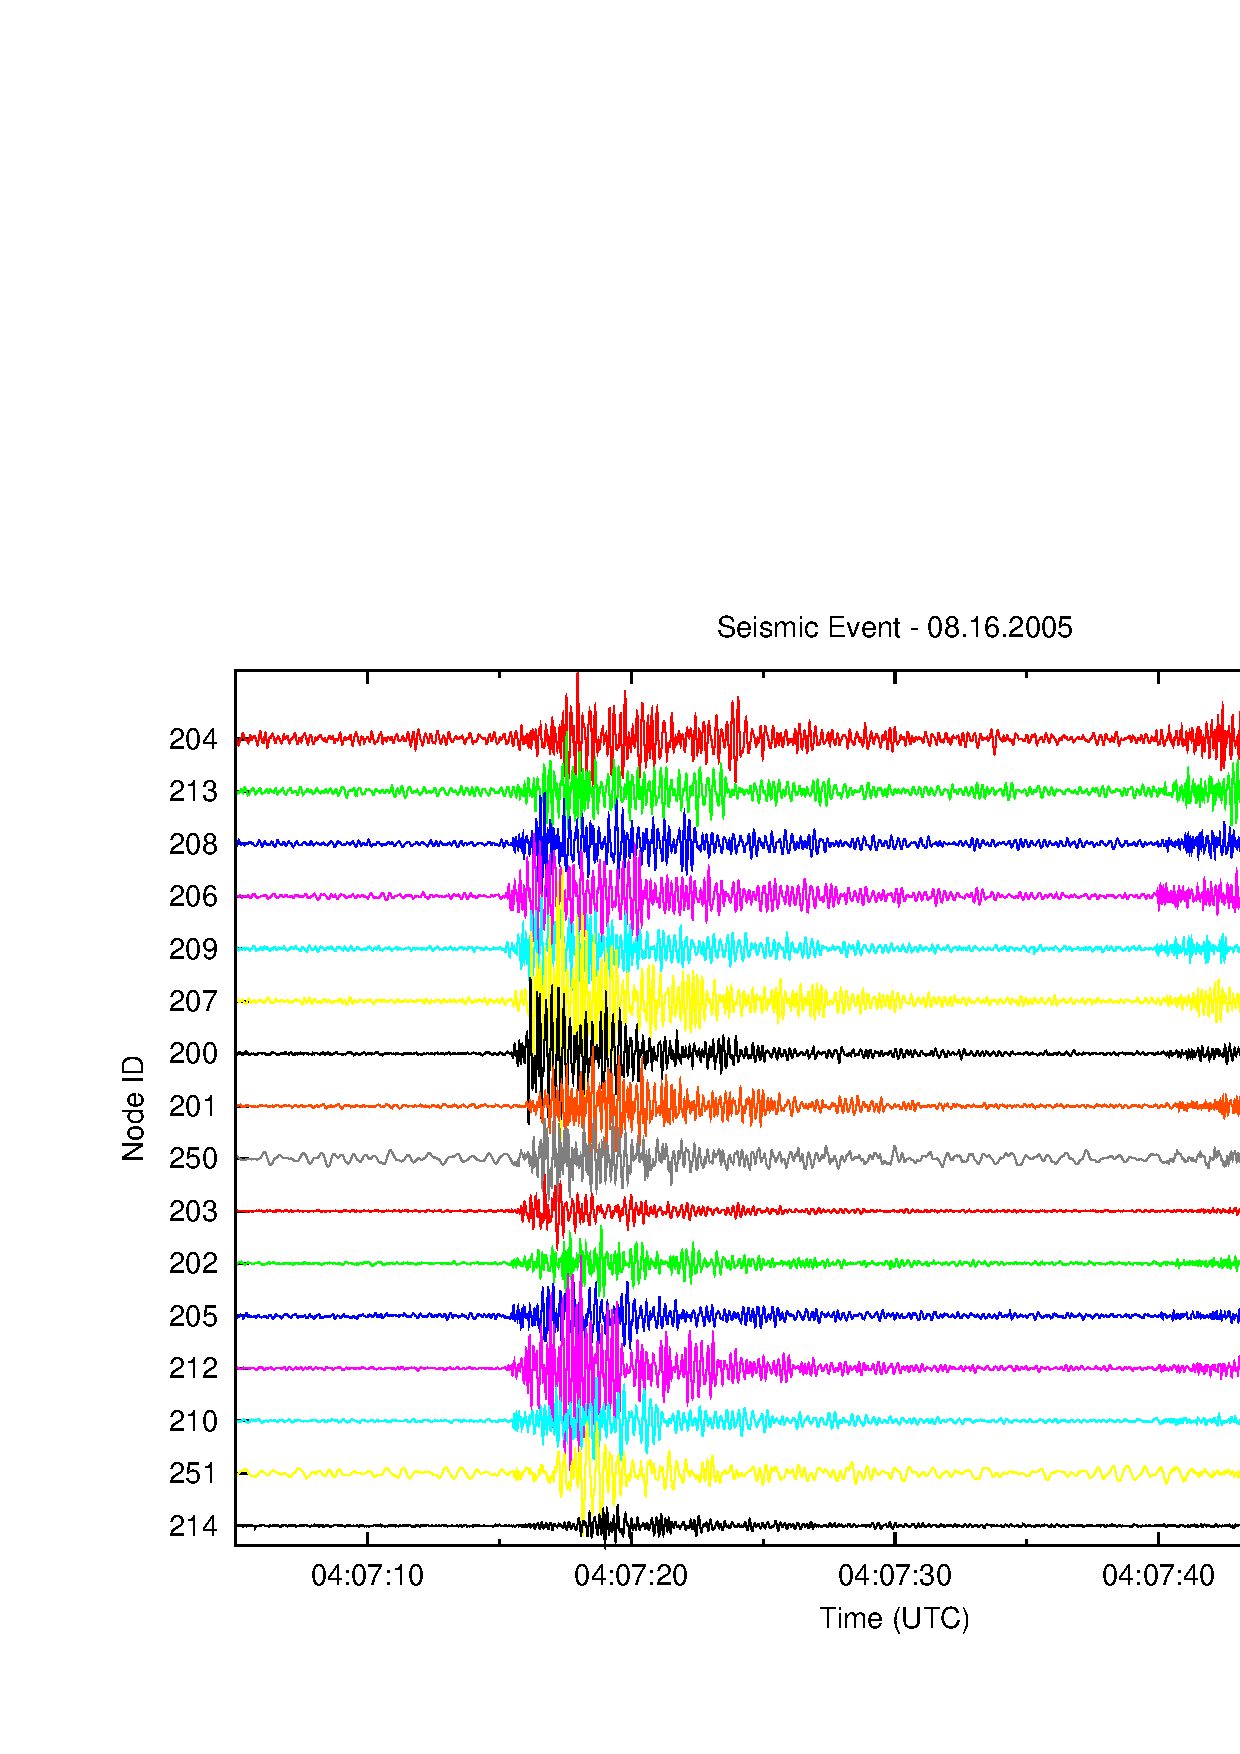
\includegraphics[width=0.7\hsize]{./figures/TEST}
\end{center}
\caption{\small {\bf {Example of an event captured by our network.  Only
seismic signals are shown.  The event shown was a Volcano Tectonic (VT) event
and had no interesting acoustic component.  Data shown has undergone several
rounds of post-processing including mapping to GMT time.}}}
\label{fig-plot}
\end{figure}

\begin{figure}[t]
\begin{center}
\includegraphics[width=0.7\hsize]{./figures/Node-212-5}
\end{center}
\caption{\small {\bf {One of our two-component stations.  The blue Pelican
Case contains the wireless sensor network node and hardware interface board.
The external antenna is mounted on the PVC pole to reduce ground effects.
A microphone is taped to the PVC pole and a single seismometer is buried
nearby.}}}
\label{fig-station2}
\end{figure}

